\documentclass[14pt]{extarticle}
%\usepackage[14pt]{extsizes} % для того чтобы задать нестандартный 14-ый размер шрифта
%\usepackage[utf8]{inputenc}
\usepackage[T1,T2A]{fontenc}
\usepackage[russian]{babel}
\usepackage{setspace,amsmath}
\usepackage[left=20mm, top=15mm, right=15mm, bottom=20mm, nohead, footskip=10mm]{geometry} % настройки полей документа
\usepackage{graphicx}
\DeclareGraphicsExtensions{.png}
%\graphicspath{{./images/}}
\usepackage{wrapfig}
\usepackage{lipsum}
\usepackage{indentfirst}

\begin{document} % начало документа
% НАЧАЛО ТИТУЛЬНОГО ЛИСТА
\begin{center}
\hfill \break
\small{\textbf{Санкт-Петербургский государственный электротехнический университет}}\\
\small{\textbf{"ЛЭТИ" им. В. И. Ульянова (Ленина)}}\\
\small{\textbf{(СПБГЭТУ "ЛЭТИ")}}\\
\hfill \break

\begin{center}
\begin{tabular}{lr}
Направление: & \textbf{27.04.04} - Управление в технических системах \\
Профиль: &  Управление и информационные технологии в технических системах \\
Факультет: & Компьютерных технологий и информатики \\
Кафедра: & Автоматики и процессов управления \\
\\
К защите допустить & \\
Зав. кафедрой &  Шестопалов М. Ю.
\end{tabular}
\end{center}

\normalsize{}
\vspace{3cm}
\large{\textbf{ВЫПУСКНАЯ КВАЛИФИКАЦИОННАЯ РАБОТА МАГИСТРА}}\\
\vspace{1cm}
\normalsize{\textbf{Тема: Параметрическое проектирование дельта-робота и решение задачи координатного управления рабочим органом}}\\
\vspace{3cm}
 
\begin{flushleft}
 \hspace{1cm} Студент \hspace{7cm} \underline{\hspace{3cm}}  О.Е. Медовиков \\ 
 \vspace{5mm}
 \hspace{1cm} Руководитель \hspace{2cm} к. т. н. \hspace{2cm} \underline{\hspace{3cm}}  С. Е. Абрамкин\\ 
 \vspace{5mm}
 \hspace{1cm} Консультант \hspace{2.3cm} к. э. н. \hspace{2cm} \underline{\hspace{3cm}}  Ю. Р. Ичкитидзе\\ 
\end{flushleft}

\vspace{2cm}
Санкт-Петербург \\ 2020 
\end{center}
\thispagestyle{empty} % выключаем отображение номера для этой страницы
 
% КОНЕЦ ТИТУЛЬНОГО ЛИСТА

\newpage
% НАЧАЛО ЗАДАНИЯ
\begin{center}
\large{\textbf{ЗАДАНИЕ НА ВЫПУСКНУЮ КВАЛИФИКАЦИОННУЮ РАБОТУ}}\\
\end{center}
\begin{flushright}
Утверждаю\\
Заф. кафедры АПУ\\
\underline{\hspace{3cm}} Шестопалов М. Ю.\\
«\underline{\hspace{0.7cm}}»\underline{\hspace{3cm}}2020 г.
\end{flushright}

\hfill \break
Студент Медовиков О. Е. \hspace{7cm} Группа 4391\\
Тема работы:\\ Параметрическое проектирование дельта-робота и решение задачи \hfill \break координатного управление рабочим органом.\\
Исходные данные (технические требования): \\
1. Написание программы для параметрического моделирования дельта-робота\\
2. Написание программы для управления дельта-роботом\\
3. Создание рабочей модели дельта-робота\\
Содержание ВКР:\\
\vspace{2cm} \\
Перечень отчетных материалов: пояснительная записка, иллюстративный\\ материал, приложение.\\
Дополнительные разделы:\\
\vspace{2cm}

\begin{tabular}{p{230pt}c}
Дата выдачи задания & Дата предоставления ВКР к защите\\
«\underline{\hspace{0.7cm}}»\underline{\hspace{3cm}}2020 г. &  «\underline{\hspace{0.7cm}}»\underline{\hspace{3cm}}2020 г.\\
\end{tabular}
\vspace{1cm}

\begin{flushleft}
 \hspace{1cm} Студент \hspace{7cm} \underline{\hspace{3cm}}  О.Е. Медовиков \\ 
 \vspace{5mm}
 \hspace{1cm} Руководитель \hspace{2cm} к. т. н. \hspace{2cm} \underline{\hspace{3cm}}  С. Е. Абрамкин\\ 
 \vspace{5mm}
 \hspace{1cm} Консультант \hspace{2.3cm} к. э. н. \hspace{2cm} \underline{\hspace{3cm}}  Ю. Р. Ичкитидзе\\
\end{flushleft}

\thispagestyle{empty} % выключаем отображение номера для этой страницы

\newpage
\begin{center}
\large{\textbf{КАЛЕНДАРНЫЙ ПЛАН ВЫПОЛНЕНИЯ ВЫПУСКНОЙ КВАЛИФИКАЦИОННОЙ РАбОТЫ}}\\
\end{center}
\begin{flushright}
Утверждаю\\
Заф. кафедры АПУ\\
\underline{\hspace{3cm}} Шестопалов М. Ю.\\
«\underline{\hspace{0.7cm}}»\underline{\hspace{3cm}}2020 г.
\vspace{1cm}
\end{flushright}

\begin{flushleft}
Студент Медовиков О. Е. \hspace{7cm} Группа 4391\\
Тема работы:\\ Параметрическое проектирование дельта-робота и решение задачи\\ координатного управление рабочим органом.\\
\vspace{1cm}
\end{flushleft}


\begin{tabular}{| c | l | c | }
\hline
№ п/п & Наименование работ & Срок выполнения\\
\hline
1 & Обзор литературы по теме работы & 10.12 - 01.02\\ 
\hline
2 & Проектирование виртуальной модели& 10.12 - 26.03\\
\hline
3 & Создание физического прототипа робота & 01.02 - 05.04\\
\hline
4 & Написание прошивки для микроконтроллера & 25.04 - 15.05 \\
\hline
5 & Создание интерфейса для управления роботом &15.05 - 25.05 \\
\hline
\end{tabular}

\vspace{3cm}

\begin{flushleft}
 \hspace{1cm} Студент \hspace{7cm} \underline{\hspace{3cm}}  О.Е. Медовиков \\ 
 \vspace{5mm}
 \hspace{1cm} Руководитель \hspace{2cm} к. т. н. \hspace{2cm} \underline{\hspace{3cm}}  С. Е. Абрамкин\\ 
 \vspace{5mm}
 \hspace{1cm} Консультант \hspace{2.3cm} к. э. н. \hspace{2cm} \underline{\hspace{3cm}}  Ю. Р. Ичкитидзе\\
\end{flushleft}

\thispagestyle{empty} % выключаем отображение номера для этой страницы


% реферат
\begin{center}
\large{\textbf{РЕФЕРАТ}}\\
\end{center}
Пояснительная записка 00 стр., 00 рис., 00 табл., 00 ист., 00 прил.\\
Ключевые слова: параметрическое моделирование, 3д печать, дельта-робот, сортировка.\\
Объект исследования:  кинематика дельта-робота.\\
Цель работы:\\
Основное содержание работы.



% аннотация на английском
\begin{center}
\large{\textbf{ABSTRACT}}\\
\end{center}
speak from my heart

% оглавление содержание
\begin{center}
\def\contentsname{СОДЕРЖАНИЕ}
\large \tableofcontents
\end{center}
% определения (не обяз)
% введение
\addcontentsline{toc}{section}{Введение}
\begin{center}
\large{\textbf{ВВЕДЕНИЕ}}\\
\end{center}
Меня зовут дундук

% основная часть
\section{Кинематика дельта-робота}
\subsection{Конструкция и устройство}
Основанием робота является база, жёстко фиксируемая в пространстве над рабочем полем. Габариты базы очерчиваются равносторонним треугольником со стороной равной f. Середины сторон треугольника обозначают координаты осей вращения рычагов и таким образом, расстояние от центра базы до оси вращения каждого рычага равно r - радиусу вписанной окружности равностороннего треугольника. Это расстояние легко находится через соотношение:
\begin{center}
f =$\frac{\sqrt{3}}{2}$  r
\end{center}

В дальнейшей работе, при описании моделирования, будут использоваться переменные с другими названиями, например, переменная rad  соответствует радиусу вписанной окружности. Это связано с удобством написания кода, так как невозможно поиском найти переменную, обозначенную одним символом, а также это неправильно, с точки зрения читаемости кода.

\begin{figure}[h!]
	\centering
	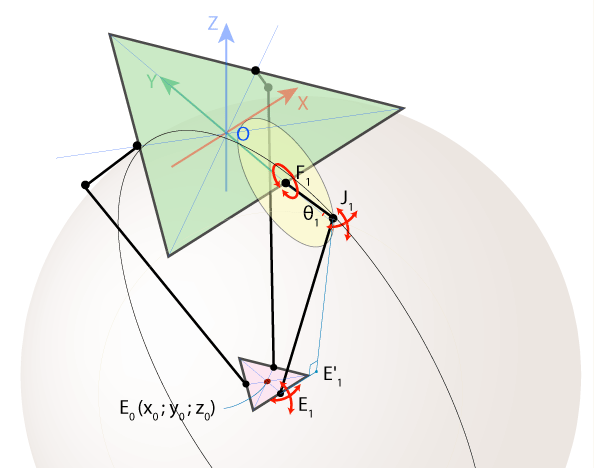
\includegraphics[width=0.8\linewidth]{./image/deltabot}
	\caption{Схематическое представление Дельта-робота}
\end{figure}

Начало координат располагается в центре базы, таким образом, чтобы Z координата высоты равнялась нулю для точек осей вращения рычагов, так как конечное расположение рабочего органа робота будет рассчитываться относительно этих координат. Три рычага нумеруются определённым образом. Первый рычаг двигается в плоскости YZ и направлен в противоположную оси Y сторону. Второй рычаг повернут относительно оси Z на 120 градусов, а третий на -120 градусов. Поворот делается по правилу правой руки, где большой палец совпадает с направлением оси Z, а согнутые пальцы показывают направление вращения. Так как робот в целом абсолютно симметричен, ошибки с нумерацией рычагов закономерны, необходимо на всех этапах строго придерживаться единому правилу обозначения рычагов.

Жёстко закреплённые каждый в своей плоскости рычаги обозначаются $r_{fi}$, а угол на который они
поворачиваются обозначают через $\theta_{i}$. Точка оси вращения рычагов обозначается как $F_{i}$, а конечная точка рычага - $J_{i}$. На конце рычага находится крепление с двумя карданными шарнирами, которое всегда параллельно стороне равностороннего треугольника, обозначающего габариты рабочего органа. Две взаимно параллельные направляющие соединяются через шарниры с вершинами треугольника, образуя параллелограмм. Из-за этого, данный робот также называют разновидностью параллельного робота.

Для математического описания робота карданные шарниры и параллельные направляющие не нужны, их заменяют рычагами обозначаемыми как $r_{ei}$. Рычаги $r_{ei}$ крепятся к серединам сторон треугольника, обозначающего габариты каретки, в которой закреплен рабочий орган. Габариты обозначаются, как и в случае с базой, равносторонним треугольником, длина стороны  которого обозначается буквой e. Координаты точек крепления карданных шарниров к каретки называют $E_{i}$, а точкой $E_{0}$ обозначается центр каретки, то-есть координата рабочего органа.

\subsection{Задача прямой кинематики дельта-робота}
Решение прямой задачи кинематики дельта-робота заключается в определении координаты центра каретки $E_{0}$ при известных углах $\theta_{i}$. Решение данной задачи необходима мне для определения координат расположения различных узлов машины, во время создания компьютерной модели. Сама идея решения достаточна проста. Так как рычаги, соединенные с двигателем, двигаются в одной плоскости, без возможности отклониться, это значит, что можно рассчитать координаты вершины рычага, зная координату оси вращения, длину рычага и угол поворота рычага. Координата конца рычагов обозначается буквой $J_{i}$. Подобным образом посчитать угол шарнира, соединяющего конец рычага и сторону каретки не представляется возможным, так как он вращается не вдоль одной плоскости, а в трёх измерениях.

Если допустить, что каретка не имеет размеров и представляет собой точку, то можно представить три сферы с центрами в $J_{i}$ и радиусами $r_{ei}$. Сферы показывают область, в которой могут теоретически могут вращаться шарниры, при данных значениях углов $\theta_{i}$. Если внести поправки на размеры каретки, точка пересечения трех сфер - будет решением, искомой координатой каретки.
\begin{figure}[h]
	\centering
	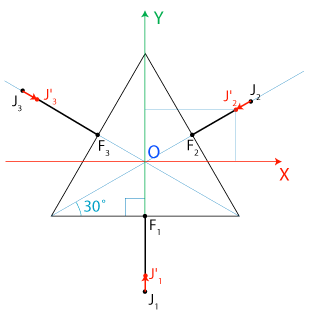
\includegraphics[width=0.4\linewidth]{./image/primay}
	\caption{Схема расчета координат рычагов}
\end{figure}

Расчет координат $J_{1}$ для первого рычага упрощается выбором системы координат. Первый рычаг параллелен оси Y и движется в плоскости YZ, поэтому координата X всегда будет равна 0. При этом Z координата оси вращения тоже равна 0, что было оговорено ранее. Значит координата $F_{1}$ будет состоять только из Y  и будет равна минус радиус вписанной окружности. В этом месте нужно взять поправку на радиус каретки, и вычесть радиус каретки из радиуса базы. Таким образом, мы сможем рассчитать точки  $J'_{i}$ - центры сфер, с общей точкой в $E_{0}$. 
\begin{center}
$t = r_{base} - r_{karet}$\\
$J'_{1} = (x_{1};y_{1};z_{1})$\\
$J'_{2} = (x_{2};y_{2};z_{2})$\\
$J'_{3} = (x_{3};y_{3};z_{3})$\\
\begin{equation*}
 \begin{cases}
        x_{1} = 0 \\
        y_{1} = -(t - r_{f}cos(\theta_{1})) \qquad\\
        z_{1} = -r_{f}cos(\theta_{1})\\
    \end{cases}
\end{equation*}
\begin{equation*}
    \begin{cases}
        x_{2} = [t+r_{f}cos(\theta_{2})]cos(30^{\circ})\\
        y_{2} = [t+r_{1}cos(\theta_{2})]sin(30^{\circ})\\
        z_{2} = -r_{f}sin(\theta_{2})\\
    \end{cases}    
\end{equation*}
\begin{equation*}
    \begin{cases}
        x_{3} = [t+r_{f}cos(\theta_{3})]cos(30^{\circ})\\
        y_{3} = [t+r_{1}cos(\theta_{3})]sin(30^{\circ})\\
        z_{3} = -r_{f}sin(\theta_{3})\\
    \end{cases}    
\end{equation*}
\end{center}

Теперь для нахождения координаты каретки, нужно решить систему из трех уравнений сфер с координатами центров в $J'_{i}$ и радиусами $r_e$.
\begin{center}
    $E_{0} = (x,y,z)$
    $( x - x_{i} )^{2} + ( y - y_{i} )^{2} + ( z - z_{i} )^{2} = r^{2}_{e} $
\end{center}

Подставим координаты $J'_{i}$, полученные ранее и получим систему уравнений вида:

\begin{equation*}
    \begin{cases}
        x^{2} + (y - y_{1})^{2} + (z - z_{1})^{2} = r^{2}_{e}\\
        (x - x_{2})^{2} + (y - y_{2})^{2} + (z - z_{2})^{2} = r^{2}_{e}\\
        (x - x_{3})^{2} + (y - y_{3})^{2} + (z - z_{3})^{2} = r^{2}_{e}\\
    \end{cases}    
\end{equation*}

Теперь раскроем скобки и немного сгруппируем переменные:

\begin{equation*}
    \begin{cases}
x^{2} + y^{2} + z^{2} - 2y_{1}y - 2z_{1}z = r^2_{e} - y^2_{1} - z^2_{1}\\
x^{2} + y^{2} + z^{2} - 2x_{2}x - 2y_{2}y - 2z_{1}z = r^2_{e} - x^2_{2} - y^2_{2} - z^2_{2}\\
x^{2} + y^{2} + z^{2} - 2x_{3}x - 2y_{3}y - 2z_{1}z = r^2_{e} - x^2_{3} - y^2_{3} -z^2_{3}\\
    \end{cases}    
\end{equation*}

Теперь можно сделать подстановку и формируем новые три уравнения, вычитая из первого сначала второе, потом третье и из второго - третье.
\begin{center}
    $\omega_{i} = x^2_{i} + y^2_{i}  + z^2_{i} $
\end{center}

\begin{equation*}
    \begin{cases}
x_{2}x + (y_{1} - y_{2})y + (z_{1} - z_{2})z = (\omega_{1} - \omega_{2})/2 \\
x_{3}x + (y_{1} - y_{3})y + (z_{1} - z_{3})z = (\omega_{1} - \omega_{3})/2 \\
(x_{2} - x_{3})x + (y_{2} - y_{3})y + (z_{2} - z_{3})z = (\omega_{2} - \omega_{3})/2 \\
    \end{cases}    
\end{equation*}

Следующим шагом вычитаем второе уравнение из первого, частично сократив $y$ выразив $x$ через $z$. Аналогично вычитаем из второго третье, частично сокращая $x$ и выражая $y$ через $z$. Так как выражения получаются очень длинными, для компактной записи вводится подстановка $a_{i},b_{i},d$.
\begin{center}
$x = a_{1}z+b_{1} \qquad  y=a_{2}z+b_{2}$\\
\end{center}

\vspace{0.75cm}
\hspace{4cm} $a_{1} =\frac{1}{d}[(z_{2}-z_{1})(y_{3}-y_{1})-(z_{3}-z_{1})(y_{2}-y_{1})]$

\hspace{4cm} $b_{1} =-\frac{1}{2d}[(\omega_{2}-\omega_{1})(y_{3}-y_{1})-(\omega_{3}-\omega_{1})(y_{2}-y_{1})]$\\
\vspace{0.75cm}

\hspace{4cm} $a_{2} =-\frac{1}{d}[(z_{2}-z_{1})x_{3}-(z_{3}-z_{1})x_{2}]$

\hspace{4cm} $b_{2} =\frac{1}{2d}[(\omega_{2}-\omega_{1})x_{3}-(\omega_{3}-\omega_{1})x_{2}]$

\vspace{0.75cm}
\hspace{4cm} $d=(y_{2}-y_{1})x_{3} - (y_{3}-y_{1})x_{2}$\\
\vspace{0.75cm}

Теперь, имея $x$ и $y$, выраженные через $z$, предстоит подставить их в уравнение сферы (например, первой) с центром в $J_{1}$, раскрыть скобки, упростить и получить:

\begin{center}
$(a^{2}_{1}+a^{2}_{2}+1)z^{2} + 2(a_{1}+a_{2}(b_{2}-y_{1})-z_{1})z +(b^{2}_{1}+(b_{2}-y_{1})^2 +z^{2}_{1}-r^{2}_{e})=0$
\end{center}

В конечном итоге задача свелась к решению квадратного уравнения, через дискриминант, корни которого будут равны $Z$ координате каретки. На данном этапе проводится проверка параметров дельта-робота. Человек произвольно задающий радиусы базы и каретки, длины рычагов и шарниров должен подобрать их в определённом соотношении, которое позволит роботу физически функционировать. Иначе, шарниры будут слишком короткими и не дотянутся до каретки. Решение уравнения выше позволяет определить физическую возможность создания робота при данных параметрах. Если дискриминант равен отрицательному числу, значит, что шарниры не дотягиваются до каретки и поэтому выбор параметров робота неверен. Если дискриминант равен 0 в рабочей области робота это приводит к неустойчивому равновесию. Эта координата называется точкой сингулярности параллельного робота, так как в её окрестностях находятся координаты с двумя равнозначными и очень близкими решениями. В окрестностях точки сингулярности управление роботом практически невозможно, так как движение вверх или вниз по оси $Z$ будет случайным. Некоторые конструкции параллельных роботов, проходя точку сингулярности, "защёлкиваются" в положение, из которого не могут выйти самостоятельно. Для правильной работы робота дискриминант должен быть большим числом, в случае моей симуляции числа достигают значений $1.4*10^{25}$ и даже больше.

\subsection{Обратная кинематика}

Задача обратной кинематики дельта-робота заключается в нахождении углов поворота рычагов $\theta_{i}$, при известной координате каретки $E_{0}=(x_{0},y_{0},z_{0})$. Данное решение основано на нахождении координат деталей первого шарнира и рычага, и вывода решения для угла $\theta_{1}$ в общем виде для первого рычага с учётом правильного расположения осей координат. Два оставшихся угла будут рассчитаны аналогично, с применением вращения оси координат на $120^{\circ}$ и $-120^{\circ}$ соответственно.

Первым шагом необходимо найти координаты крепления шарнира к каретке. Эта точка находится на стороне равностороннего треугольника и смещена от точки $E_{0}$ на величину радиуса вписанной окружности.

\begin{center}
$E_{1} (x_{0},y_{0}-\frac{e}{2\sqrt{3}},z_{0})$
\end{center}

Так как в общем виде каретка будет иметь некое смещение по оси $X$, а это значит, что шарнир и рычаг не будут лежать в одной плоскости $YZ$. Для решения необходимо найти проекцию шарнира на плоскость $YZ$. Верхняя точка проекции шарнира совпадает с координатой конца рычага $J_{1}$, а нижняя точка обозначается $E'_{0}$. 

\begin{center}
$E'_{1} (0,y_{0}-\frac{e}{2\sqrt{3}},z_{0})$
\end{center}

Соответственно длинна проекции шарнира находится по теореме Пифагора:

\begin{center}
$E'_{1}J_{1} = \sqrt{(E_{1}J_{1})^{2} -(E_{1}E'_{1})^{2}}  $
\end{center}

Так как гипотенуза равна длине шарнира, а меньший катет - смещению каретки по $X$, то: 

\begin{center}
    $E'_{1}J_{1} = \sqrt{r^{2}_{e} - x^{2}_{0} }  $
\end{center}

Напомню, что координата оси вращения первого рычага $F_{1}$  смещена от центра координат на радиус вписанной окружности, таким же образом, как и крепление шарнира каретки.

\begin{center}
    $F_{1}(0,\frac{-f}{2\sqrt{3}},0)$
\end{center}

Теперь есть все необходимое, для нахождения координаты соединения рычага с шарниром $J_{1}$. Вращаясь рычаг описывает окружность с радиусом $r_{f}$ и центром в  $F_{1}$. Проекция шарнира вращаясь описывает окружность с найденным выше радиусом $E'_{1}J_{1}$ и центром в $E'_{1}$. Найдя точки пересечения этих двух окружностей, мы получим две физически возможные координаты точки соединения рычага и шарнира, одна из которых ложная, а вторая (наименьшая по $Y$) истинная. Общие точки находятся путём решения решения системы уравнений двух окружностей.

\begin{equation*}
    \begin{cases}
        (y_{J_{1}} -y_{F_{1}})^{2} +(Z_{J_{1}}-z_{F_{1}})^{2} = r^{2}_{f}\\
        (y_{J_{1}} -y_{E'_{1}})^{2} +(Z_{J_{1}}-z_{E'_{1}})^{2} = r^{2}_{e}-x_{0}\\
    \end{cases}
\end{equation*}

Подставляем известные координаты центров окружностей:


\begin{equation*}
    \begin{cases}
        (y_{J_{1}} + \frac{f}{2\sqrt{3}})^{2} + z^{2}_{J_{1}} = r^{2}_{f}\\
        (y_{J_{1}} -y_{0} +\frac{e}{2\sqrt{3}})^{2} +(z_{J_{1}} -z_{0})^{2} = r^{2}_{e}-x_{0}\\
    \end{cases}
\end{equation*}

 В данном случае, так как мы работаем с окружностями и игнорируем ось $X$, получается система из двух уравнений с двумя неизвестными. Если раскрыть скобки и вычесть из первого уравнения второе, то можно выразить $z$ через $y$ и подставить во второе уравнение, получив квадратное уравнение.

 \begin{center}
\vspace{0.75cm}
 $\frac{x^{2}_{0}+y^{2}_{0}+z^{2}_{0}+r^{2}_{e}+r^{2}_{f} -y^{2}_{F_{1}} }{2z_{0}}y^{2} - \frac{y_{F_{1}}-y_{0}}{z_{0}}y = 0$
\end{center}







\section{Моделирование робота}
\subsection{База}
бла бла


% заключение
\addcontentsline{toc}{section}{Заключение}
\begin{center}
\large{\textbf{ЗАКЛЮЧЕНИЕ}}\\
\end{center}
Бла-бла-бла просто гений

% список источников
\addcontentsline{toc}{section}{Список}
\begin{center}
\large{\textbf{СПИСОК ИСПОЛЬЗОВАННЫХ ИСТОЧНИКОВ}}\\
\end{center}
1. какая-то статья 


% приложения (не обязательно)

\end{document}
